\documentclass[a4paper,10pt,twocolumn]{article}
\usepackage[T1]{fontenc}
\usepackage[utf8]{inputenc}
\usepackage{lmodern}
\usepackage{amsmath,amssymb}
\usepackage{graphicx}
\usepackage{booktabs}
\usepackage{multirow}
\usepackage{array}
\usepackage{url}
\usepackage{xcolor}
\usepackage{microtype}
\usepackage[margin=1.8cm,columnsep=0.6cm]{geometry}
\usepackage[hidelinks]{hyperref}
\usepackage{caption}
\captionsetup{font=footnotesize,labelfont=bf}
\setlength{\parskip}{0.18em}
\setlength{\parindent}{1em}
\setlength{\textfloatsep}{9pt plus 2pt minus 2pt}
\setlength{\floatsep}{8pt plus 2pt minus 2pt}
\setlength{\intextsep}{8pt plus 2pt minus 2pt}
\renewcommand{\arraystretch}{1.08}
\title{\vspace{-1.35cm}\bfseries A Reproducible Comparison of Tabular Q-Learning, DQN, and Double DQN on Gymnasium Classic Control Environments\\[3pt]
\large Experimental Study and Failure-Mode Analysis}
\author{\textbf{Kevin Erazo} \quad \textbf{Steven Rodríguez}\\
\small Intelligent Agents --- Project 01 \quad | \quad October 2026}
\date{}
\begin{document}
\maketitle
\vspace{-1.0cm}
\begin{abstract}
We implement tabular Q-learning, Deep Q-Networks (DQN), and Double DQN without prebuilt reinforcement-learning agents and compare them experimentally in Gymnasium. Tier~1 evaluates three uniform state discretizations (6, 10, and 20 bins per observation dimension) against DQN on CartPole-v1 under 200,000 training steps per run. Tier~2 studies two DQN hyperparameters and removal of the target network on Acrobot-v1; Tier~3 compares vanilla DQN against Double DQN on the same environment. Each configuration uses three independent seeds and a final greedy evaluation of 100 episodes. On CartPole, tabular Q-learning with 20 bins obtains the highest final across-seed mean (280.87), whereas DQN reaches 117.46 despite stronger initial performance. On Acrobot, Double DQN averages $-269.38$, compared with $-371.05$ for vanilla DQN, but both are highly variable. Four of 33 runs meet the project-specific final evaluation thresholds; no configuration succeeds for all three seeds. These results highlight the difference between early learning, terminal checkpoint performance, and robust multi-seed success.
\end{abstract}
\noindent\textbf{Keywords:} reinforcement learning; tabular Q-learning; DQN; Double DQN; reproducibility; ablation.

\section{Introduction}
Reinforcement learning (RL) studies agents that choose actions in order to maximize long-term cumulative reward by interacting with an environment. The classical action-value approach represents a function $Q(s,a)$, the expected discounted return of selecting action $a$ in state $s$ and following a policy thereafter. Tabular Q-learning stores the function explicitly, which is practical only when the set of relevant states and actions is small. Deep Q-Networks (DQN) instead learn a function approximator $Q_\theta(s,a)$, permitting direct use of low-dimensional continuous observations as inputs when actions remain discrete \cite{sutton2018,mnih2015}.

Function approximation does not guarantee better performance: replayed data, changing value targets, exploration schedules, and optimization choices can destabilize learning. Double DQN addresses a particular source of error by separating next-action selection and evaluation in the target \cite{vanhasselt2016}. We therefore study not only final scores but learning behavior, sensitivity to design choices, and cross-seed variance.

Our research questions are: (RQ1) How do tabular discretization and DQN compare on CartPole under equal environment-step budgets? (RQ2) How sensitive is DQN on Acrobot to learning rate, exploration decay, and the target network? (RQ3) Does Double DQN improve the final performance and consistency of vanilla DQN? The experiments follow the course project's thresholds, not claims of general-purpose convergence.

\section{Environments and algorithm suitability}
\textbf{CartPole-v1} has four continuous observation components and two discrete actions. The task rewards the agent for keeping a pole balanced; episodes last at most 500 steps. The course requires a 100-episode greedy mean of at least 475. The currently documented Gymnasium default reference differs from this course threshold, so we explicitly adopt the latter \cite{gymcart}.

\textbf{Acrobot-v1} has six continuous observation components and three discrete actions. Its negative step-based return encourages reaching the terminal height promptly, with a maximum of 500 steps per episode. The project threshold is a mean return of at least $-100$ on 100 greedy episodes \cite{gymacro}. Unlike standard tabular Q-learning, a neural network can use its observation vector without discretizing each feature.

These two environments are appropriate for ordinary DQN because the set of actions is finite. They also create a useful contrast: CartPole's dense survival reward and Acrobot's harder swing-up task have different exploration and stability demands. The analysis-only section later examines why the same approach cannot be transferred unmodified to high-dimensional continuous-action locomotion.

\section{Algorithms}
\subsection{Tabular Q-learning}
We map the four CartPole observations to an integer state using equal-width bins. All dimensions use the same bin count $b\in\{6,10,20\}$. Finite clipping ranges are, respectively, $[-2.4,2.4]$ for cart position, $[-3,3]$ for cart velocity, $[-0.2095,0.2095]$ for pole angle, and $[-3.5,3.5]$ for angular velocity. These are explicit engineering choices rather than a claim that the velocities are naturally bounded. There are $b^4$ discrete states: 1,296; 10,000; and 160,000.

For transition $(s,a,r,s')$, the tabular update is
\begin{equation}
Q(s,a) \leftarrow Q(s,a)+\alpha\big[r+\gamma(1-d)\max_{a'}Q(s',a')-Q(s,a)\big],
\label{eq:ql}
\end{equation}
where $d=1$ for a true MDP termination, $\alpha=0.1$, and $\gamma=0.99$. We initialize values to zero, and use $\epsilon$-greedy action selection with a linear decrease from 1.0 to 0.05 over the first 80\% of training steps. At evaluation time, $\epsilon=0$.

\subsection{DQN and Double DQN}
The DQN policy is an MLP with two hidden ReLU layers of width 128. The network has four inputs and two outputs on CartPole, and six inputs and three outputs on Acrobot. Unless otherwise stated, $\gamma=0.99$, Adam learning rate $5\times10^{-4}$, minibatch size 64, replay capacity 50,000, one gradient step every four environment transitions, and a 1,000-step learning warmup. Hard target-network updates occur every 1,000 steps, with gradient norm clipping at 10. Exploration decays linearly from $\epsilon=1$ to 0.05 over 50\% of the training budget.

For vanilla DQN the bootstrapped target is
\begin{equation}
y_{\rm DQN}=r+\gamma(1-d)\max_{a'}Q_{\theta^-}(s',a'),
\end{equation}
where $\theta^-$ are periodically synchronized target parameters. The online network minimizes the smooth $L_1$ loss on replayed transitions. In the target-network ablation, the online network supplies next-action values instead, under $\texttt{no\_grad}$. Replay remains enabled, so the ablation isolates removal of the target network rather than changing several components at once.

Double DQN changes only the target computation:
\begin{equation}
\begin{split}
y_{\rm DDQN} = r+\gamma(1-d)Q_{\theta^-}\big(s',\\
\arg\max_{a'}Q_{\theta}(s',a')\big).
\end{split}
\end{equation}
The online parameters select the next action; target parameters evaluate it. This aims to mitigate maximization-related overestimation, but our run logs do not record estimated-versus-true Q-values, so any mechanism-level explanation remains a hypothesis rather than a directly measured effect.

The implementation distinguishes environment termination from time-limit truncation. Either event ends an episode, but only a true termination suppresses bootstrapping. This is important for consistent Bellman targets in Gymnasium's API \cite{gymapi}.

\section{Experimental protocol and reproducibility}
All algorithms were implemented in Python/NumPy/PyTorch. Recorded software versions are Python 3.14.4, Gymnasium 1.4.0, and PyTorch 2.15.0+cu132 with \texttt{device=cpu}. Experiments were executed on a laptop with Intel Core i5-1135G7 CPU and 12 GB RAM. Although the installed PyTorch build includes CUDA dependencies, the logged training device is CPU.

We use seeds 0, 1, and 2 for every configuration. Each Tier~1 run receives exactly 200,000 environment interactions; Tier~2 and Tier~3 runs receive 100,000. All methods are evaluated greedily every 10,000 steps for ten episodes; a final greedy evaluation uses 100 episodes, independently from the training environment. Evaluation start states follow reproducible seeded resets. Per-seed training episodes, periodic evaluations, final metrics, model checkpoints, and execution times are preserved in the results package.

We report cross-seed mean and sample standard deviation of \emph{per-seed 100-episode final means}; this is different from the within-seed variation across its 100 episodes. The shaded periodic-learning bands show $\pm1$ sample standard deviation across the three independent seeds. They are descriptive uncertainty bands, not confidence intervals. Success is counted only when a final 100-episode mean passes the course threshold. A temporary crossing on a ten-episode periodic evaluation is designated \emph{provisional}, not a validated success.

The Tier~2 learning-rate sweep uses $\{10^{-4},5\times10^{-4},10^{-3}\}$ with the middle value as baseline. The exploration-decay sweep uses 20\%, 50\%, and 80\% of training steps. One factor is varied at a time around the shared baseline. A no-target-network ablation and a Double DQN extension use the same environment, step budget, and seeds as vanilla DQN.

\begin{table*}[t]
\centering\small
\caption{Final 100-episode greedy return by seed in CartPole-v1. All runs use 200,000 training steps. Across-seed standard deviations are sample standard deviations; larger returns are better.}
\label{tab:cartpole}
\begin{tabular}{lrrrrrc}
\toprule
Method & Seed 0 & Seed 1 & Seed 2 & Across-seed mean & Across-seed SD & Threshold passes \\
\midrule
Q-learning (6 bins) & 205.01 & 145.34 & 135.04 & 161.80 & 37.78 & 0/3 \\
Q-learning (10 bins) & 139.58 & \textbf{497.22} & 190.24 & 275.68 & 193.52 & 1/3 \\
Q-learning (20 bins) & 199.16 & 428.33 & 215.11 & \textbf{280.87} & 127.96 & 0/3 \\
DQN & 92.49 & 156.77 & 103.13 & 117.46 & 34.45 & 0/3 \\
\bottomrule
\end{tabular}
\end{table*}

\section{Tier 1 results: CartPole}
Table~\ref{tab:cartpole} reports the final results. The largest final mean is obtained by 20-bin tabular Q-learning (280.87), closely followed by 10-bin tabular Q-learning (275.68). Their means differ by 5.19 points, much less than their cross-seed variability. Therefore, a claim that 20 bins is reliably superior is not supported. The 10-bin configuration reaches 497.22 in seed 1 and is the only CartPole configuration to pass the 475 threshold in a final 100-episode evaluation; neither 10 bins nor any other configuration passes in all three seeds.

\begin{figure*}[t]
\centering
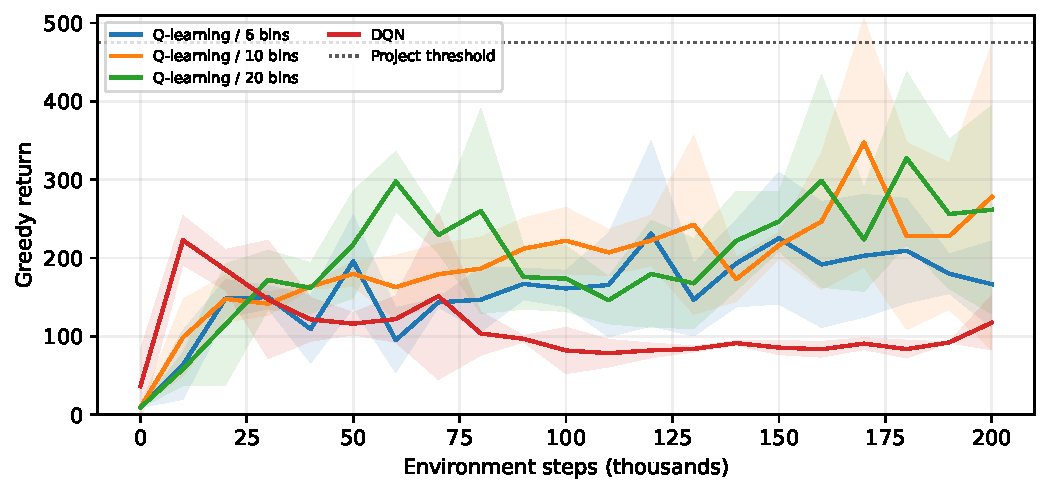
\includegraphics[width=0.89\textwidth]{paper_figures/cartpole_evaluations.pdf}
\caption{Tier~1 periodic greedy evaluations from the archived ten-episode measurements. Lines are means over three seeds; shaded regions are $\pm1$ sample SD across seeds. The dotted line marks the project target of 475. Final 100-episode outcomes are reported separately in Table~\ref{tab:cartpole}.}
\label{fig:cartpolecurves}
\end{figure*}

Early learning and final stability tell different stories (Fig.~\ref{fig:cartpolecurves}). At 10,000 steps, DQN's average periodic return is 222.80, compared with 63.63, 98.63, and 58.23 for the 6-, 10-, and 20-bin tabular agents. Thus DQN initially learns faster in terms of environment interactions on this particular setup. However, its average periodic return declines to 82.07 by step 100,000 and its final 100-episode mean is only 117.46. By contrast, the two finer tabular configurations achieve better final means. The early DQN advantage does not imply convergence or better terminal performance.

The tabular discretization results reflect a coverage--resolution trade-off. Coarse bins pool observations that may require different actions; fine bins distinguish more states but require more visits per state. Increasing from 6 to 20 bins multiplies the size of the table by a factor of about 123.5. Yet the measured final ranking is not monotonic across seeds, so the role of bins should not be reduced to ``more bins is always better.'' The particular clipping bounds and randomized learning trajectories are material limitations.

DQN's consistent late decline deserves further study, but the present logs alone cannot attribute it to target-network updates, overestimated Q-values, or the learning rate. These logs include evaluation returns and final network weights, but not temporal-difference errors, estimated Q distributions, or intermediate checkpoints. This distinction avoids presenting a plausible mechanism as an observed fact.

\section{Tier 2 results: Acrobot DQN and ablation}
\begin{table*}[t]
\centering\small
\caption{Acrobot-v1 results: each configuration has 100,000 training steps per seed and 100 greedy evaluation episodes at the end. Negative returns closer to zero are better; the project threshold is $-100$.}
\label{tab:acrobot}
\begin{tabular}{lrrrrrc}
\toprule
Method/configuration & Seed 0 & Seed 1 & Seed 2 & Across-seed mean & Across-seed SD & Threshold passes \\
\midrule
DQN baseline & -113.15 & -500.00 & -500.00 & -371.05 & 223.35 & 0/3 \\
DQN, LR $10^{-4}$ & -176.46 & -500.00 & \textbf{-86.29} & \textbf{-254.25} & 217.55 & 1/3 \\
DQN, LR $10^{-3}$ & -500.00 & -119.12 & -500.00 & -373.04 & 219.90 & 0/3 \\
DQN, $\epsilon$-decay 20\% & -500.00 & -500.00 & -500.00 & -500.00 & 0.00 & 0/3 \\
DQN, $\epsilon$-decay 80\% & -500.00 & -500.00 & \textbf{-85.15} & -361.72 & 239.51 & 1/3 \\
DQN, no target network & -500.00 & -500.00 & -500.00 & -500.00 & 0.00 & 0/3 \\
\midrule
Double DQN (Tier 3) & -213.49 & \textbf{-94.64} & -500.00 & -269.38 & 208.38 & 1/3 \\
\bottomrule
\end{tabular}
\end{table*}

Table~\ref{tab:acrobot} shows that DQN on Acrobot is strongly sensitive to configuration and seed. Of the Tier~2 candidates, LR $10^{-4}$ has the highest across-seed final mean ($-254.25$) but ranges from $-500.00$ to $-86.29$. The larger learning rate $10^{-3}$ scores $-373.04$, near the baseline mean $-371.05$. Thus the lower learning rate was better \emph{on average in these runs}, not reliably better in every seed.

Short exploration decay (20\%) performs poorly: each final evaluation yields $-500.00$. A longer decay (80\%) succeeds for seed 2 with $-85.15$, yet fails for seeds 0 and 1. Taken together, these results suggest that exploration schedule influences whether a useful policy is found and retained, but the sample is too small to identify a universally effective schedule.

Removing the target network results in $-500.00$ across all three final seeds. At intermediate checkpoints some policies briefly showed returns above $-100$ in ten-episode tests, but this did not persist at the final assessment. The ablation is therefore consistent with a stabilizing role for a target network on this design; it does \emph{not} prove that target networks always improve every DQN run. Experience replay remained enabled for both conditions, so its specific causal contribution was not ablated here.

\begin{figure*}[t]
\centering
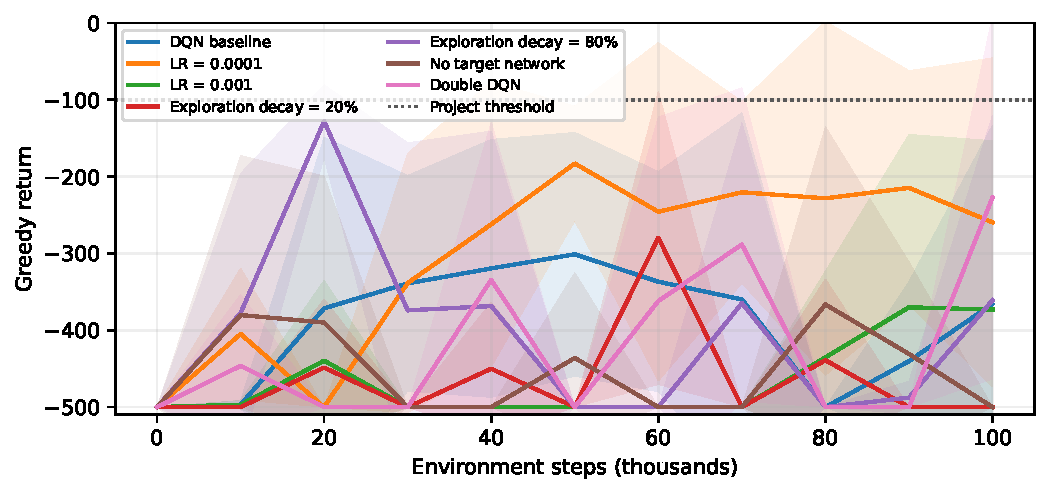
\includegraphics[width=0.89\textwidth]{paper_figures/acrobot_evaluations.pdf}
\caption{Periodic ten-episode evaluations in Acrobot-v1: baseline DQN, two learning-rate changes, two exploration-decay changes, the no-target ablation, and Double DQN. Each curve averages three seeds with $\pm1$ SD bands. Abrupt improvements and subsequent regressions should not be confused with verified 100-episode success.}
\label{fig:acrobotcurves}
\end{figure*}

The time series in Fig.~\ref{fig:acrobotcurves} shows frequent large changes, including returns that move from near the $-100$ goal back to $-500$. This is partly visible in the baseline seed 1 (periodic $-79.6$ at 70,000 steps; final $-500$) and in the no-target experiment. Since only the terminal weights were saved, final evaluations test the last policy rather than the best intermediate policy. This checkpoint policy is a protocol choice, not proof that best-checkpoint selection would produce stable behavior across unseen episodes.

\section{Tier 3: Double DQN versus vanilla DQN}
Double DQN achieves a final mean of $-269.38$ and sample SD of 208.38; vanilla DQN achieves $-371.05$ and SD 223.35. The across-seed mean improvement is 101.67 points, but the paired differences (Double DQN minus DQN) for seeds 0, 1, and 2 are $-100.34$, $+405.36$, and $0.00$. This uneven distribution is more informative than the aggregate alone. Double DQN is worse in one seed, much better in another, and equally unsuccessful in the third. Its observed success count is 1/3 versus 0/3 for the baseline.

\begin{figure}[t]
\centering
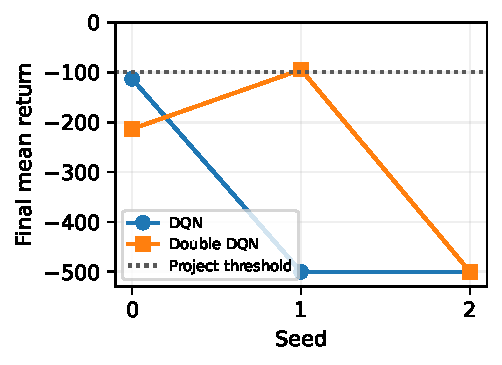
\includegraphics[width=\columnwidth]{paper_figures/paired_double_dqn.pdf}
\caption{Matched-seed final comparison between vanilla and Double DQN on Acrobot. Higher returns are better.}
\label{fig:paired}
\end{figure}

The cross-seed sample size is only three. Hence neither a statistically robust improvement nor a reduction in value overestimation can be asserted from these rewards alone. Nevertheless, the extension meets the assignment's comparative objective and reveals a testable hypothesis: alternative target estimators may affect whether learned behavior survives continued updates.

\section{Compute cost, limitations, and next tests}
The archived logs total 4.5 million training environment interactions and 1,229.97 seconds (20.50 minutes) of per-run wall-clock time, including evaluation. Tier~1 represents 12 runs, Tier~2 18, and Tier~3 three. Average per-run wall times are about 23--24 s for tabular CartPole, 59.74 s for CartPole DQN, and 36.60--41.72 s for Acrobot configurations. These measurements depend on the recorded CPU platform and should not be generalized to other hardware. Auxiliary plotting and GIF creation are not included in the summed run timers.

Limitations include only three seeds, ten-episode periodic evaluations, nonidentical exploration-decay settings between tabular and DQN baselines, fixed uniform discretization bounds, and storage of only the final policy. No gradient-loss series, Q-value diagnostics, replay-distribution statistics, or independent post-selection hold-out evaluation was recorded. The 100-episode final evaluations offer stronger evidence than a ten-episode snapshot, but 100 episodes from one terminal network are not a substitute for robust results across independently trained agents.

A controlled follow-up should preserve this initial experiment unmodified, log loss and Q-value statistics, optionally compare smaller learning rates and target update intervals, and save a best-intermediate checkpoint using one validation set while evaluating it on a \emph{different} held-out seed set. This future work is proposed only; no such results appear in the submitted archive.

\section{Analysis-only: limits of tabular RL and discrete-action DQN}
\subsection{Continuous-action locomotion}
The original project requires an analysis of tasks deliberately excluded from implementation: BipedalWalker-v3, Hopper-v5, HalfCheetah-v5, and Ant-v5. These tasks expose real-valued action vectors. Standard DQN predicts one action value per \emph{discrete} action; without action discretization or architectural changes, its output cannot directly represent the continuous torque vector. Tabular learning additionally struggles with high-dimensional continuous observations \cite{bipedaldocs,hopperdocs,halfdocs,antdocs}.

For the documented default configurations, BipedalWalker has 24 observation components and 4 action coordinates; Hopper has 11 and 3; HalfCheetah has 17 and 6; Ant has 105 and 8. Even assigning just ten discrete bins to each BipedalWalker observation creates up to $10^{24}$ tabular states before considering actions. This makes thorough state-action visitation and reliable table estimation implausible under ordinary data budgets.

If each of $d$ action coordinates is replaced by $k$ discrete choices, the joint action set has $k^d$ elements. This exponential scaling is not specific to any network implementation. For example, with just five choices per coordinate, the complete action grids contain 625 actions (BipedalWalker), 125 (Hopper), 15,625 (HalfCheetah), and 390,625 (Ant). At eleven choices per coordinate, those become 14,641, 1,331, 1,771,561, and 214,358,881 actions, respectively. A conventional DQN would need one predicted value per discrete joint action. Such output sizes can make both exploration and action maximization prohibitively expensive. Conversely, coarse torque bins may not express the fine coordination needed for locomotion. These counts are a \emph{theoretical discretization thought experiment}, not measured runtimes or trained policies.

\subsection{Continuous-control algorithm families}
\textbf{Proximal Policy Optimization (PPO)} uses an actor-based policy, commonly a continuous action distribution, with a clipped policy objective to limit the impact of updates \cite{ppo2017}. Its on-policy character tends to require new rollouts when updating, although implementation simplicity and stable improvement are attractive for many physics environments.

\textbf{Soft Actor-Critic (SAC)} is an off-policy actor-critic approach. A continuous stochastic policy can output real-valued actions; replayed experience reduces the dependence on new interaction samples, and entropy regularization supports broader exploration \cite{sac2018}. Sample efficiency and computational efficiency are separate concepts, so replay alone does not guarantee low wall time.

\textbf{Twin Delayed Deep Deterministic Policy Gradient (TD3)} uses a deterministic actor for continuous actions, twin critics, delayed actor updates, and target-policy smoothing to alleviate approximation problems \cite{td32018}. Its design targets sources of instability different from the discrete-action Double DQN target in this report. PPO, SAC, and TD3 still require tuning and empirical evaluation, but do not enumerate the full Cartesian action grid as ordinary DQN would.

\subsection{High-dimensional visual observations}
Atari Pong has a different obstacle to tabular RL: pixel-based observations. An RGB image of $210\times160\times3$ contains 100,800 scalar channel values. If each channel were merely binary, the observation space could already contain up to $2^{100800}$ distinct raw encodings. Exact tabular lookup cannot generalize across visually similar frames, and training trajectories visit only a negligible fraction of such possibilities. A pixel-based DQN instead relies on convolutional features, image preprocessing, and often stacked frames to infer motion from visual observations \cite{mnih2015,aledocs}. The substantial computational and memory demands explain why the assignment treats this as an optional GPU track rather than a mandatory laptop experiment.

Taken together, these examples show that algorithm choice depends jointly on observation representation, action structure, computational budget, and the desired level of generalization. Tabular Q-learning can be defensible for discretized classic control, ordinary DQN for modest discrete action spaces, and continuous-action actor-critic methods for complex torque control.

\section{Conclusion}
The project achieved the planned comparisons and stored reproducible traces for 33 training runs, yet no configuration reached its project-specific final threshold in every seed. On CartPole, DQN exhibited promising early sample efficiency but weaker terminal performance than the two finer tabular alternatives. On Acrobot, lower DQN learning rate and Double DQN improved the average outcome under some conditions, without establishing robust multi-seed success. The target-network ablation failed in all terminal evaluations. Such negative and mixed results are informative when supported by raw logs and explicit statistical limitations. Future experiments should focus on retention of good policies, better monitoring of learning dynamics, and separate validation versus test evaluations.

\section*{Reproducibility and AI-use statement}
All numerical results are calculated from the supplied experiment archives. Reproduction commands from the repository include \texttt{python -m scripts.run\_experiments --suite tier1}, \texttt{--suite tier2}, and \texttt{--suite tier3}, followed by \texttt{python -m scripts.plot\_results --suite all}. Default seed list is \texttt{0 1 2}; results are saved to \texttt{results/full}. Exact software versions, network settings, checkpoint names, and evaluation logs appear in each run's JSON summary. The public repository also contains the complete per-run metrics, saved checkpoints, figures, and two real-environment agent GIFs (\url{https://github.com/Steven735-star/rl-benchmark-lab}).

OpenAI ChatGPT assisted with planning, Python/PyTorch implementation, testing, experiment interpretation, visualization, and report drafting. The human team executed the Gymnasium experiments and supplied the measured logs. Both students must verify all reported claims, citations, and numerical summaries; understand and defend the code and figures; and review the representative reconstructed prompts presented in Appendix A. The reconstructed wording should be replaced by original transcripts wherever available.

\begin{thebibliography}{12}\footnotesize
\bibitem{sutton2018} R. S. Sutton and A. G. Barto. \emph{Reinforcement Learning: An Introduction}, 2nd ed. MIT Press, 2018.
\bibitem{mnih2015} V. Mnih et al. Human-level control through deep reinforcement learning. \emph{Nature}, 518:529--533, 2015. doi:10.1038/nature14236.
\bibitem{vanhasselt2016} H. van Hasselt, A. Guez, and D. Silver. Deep reinforcement learning with Double Q-learning. \emph{AAAI}, 2016. doi:10.1609/aaai.v30i1.10295.
\bibitem{gymcart} Farama Foundation. Cart Pole, Gymnasium documentation. \url{https://gymnasium.farama.org/environments/classic_control/cart_pole/}.
\bibitem{gymacro} Farama Foundation. Acrobot, Gymnasium documentation. \url{https://gymnasium.farama.org/environments/classic_control/acrobot/}.
\bibitem{gymapi} Farama Foundation. Gymnasium Step API. \url{https://gymnasium.farama.org/introduction/migration_guide/}.
\bibitem{bipedaldocs} Farama Foundation. Bipedal Walker, Gymnasium documentation. \url{https://gymnasium.farama.org/environments/box2d/bipedal_walker/}.
\bibitem{hopperdocs} Farama Foundation. Hopper, Gymnasium documentation. \url{https://gymnasium.farama.org/environments/mujoco/hopper/}.
\bibitem{halfdocs} Farama Foundation. Half Cheetah, Gymnasium documentation. \url{https://gymnasium.farama.org/environments/mujoco/half_cheetah/}.
\bibitem{antdocs} Farama Foundation. Ant, Gymnasium documentation. \url{https://gymnasium.farama.org/environments/mujoco/ant/}.
\bibitem{ppo2017} J. Schulman et al. Proximal policy optimization algorithms. arXiv:1707.06347, 2017.
\bibitem{sac2018} T. Haarnoja et al. Soft actor-critic: Off-policy maximum entropy deep reinforcement learning with a stochastic actor. \emph{ICML}, 2018.
\bibitem{td32018} S. Fujimoto, H. van Hoof, and D. Meger. Addressing function approximation error in actor-critic methods. \emph{ICML}, 2018.
\bibitem{aledocs} Farama Foundation. Arcade Learning Environment, Pong. \url{https://ale.farama.org/environments/pong/}.
\end{thebibliography}

\section*{Appendix A: Representative Generative-AI Prompts}
\noindent\textit{Disclosure note.} The following prompts are reconstructed examples of the main requests corresponding to the AI-assisted tasks disclosed above. They are not verbatim transcripts, and their precise wording has not been independently verified. The team should replace any entry with the original prompt if the conversation record is available.
\begin{enumerate}
\setlength{\itemsep}{1pt}
\setlength{\parskip}{0pt}
\item \textbf{Experimental design:} ``Propose a reproducible comparison of tabular Q-learning and DQN on CartPole-v1 and a DQN sensitivity study on Acrobot-v1. Use three independent seeds, fixed environment-step budgets, and separate training from greedy evaluation.''
\item \textbf{Tabular agent:} ``Implement tabular Q-learning for CartPole-v1 in Python and NumPy with 6, 10, and 20 bins per observation dimension, epsilon-greedy exploration, and explicit treatment of termination versus time-limit truncation.''
\item \textbf{Deep RL agents:} ``Implement DQN and Double DQN directly in PyTorch, including a replay buffer, target network, epsilon schedule, Huber loss, gradient clipping, and an ablation that disables the target network. Do not use prebuilt RL agents.''
\item \textbf{Experimental pipeline:} ``Create command-line scripts to run the defined configurations for seeds 0, 1, and 2; log per-episode returns, ten-episode greedy checkpoints, final 100-episode evaluations, hyperparameters, elapsed time, and saved models.''
\item \textbf{Analysis and visualization:} ``Aggregate measured results across seeds using sample standard deviation. Plot learning curves versus environment steps with uncertainty bands, compare final returns and training time, and do not fabricate missing measurements.''
\item \textbf{Scientific interpretation and writing:} ``Help organize a concise double-column report discussing sample efficiency, discretization, hyperparameter sensitivity, the target-network ablation, and Double DQN. Explain negative results and limitations without claiming unsupported convergence or causal mechanisms.''
\end{enumerate}

\end{document}